\chapter{Business Analysis}\label{chap:business_analysis}

  \section{Knowledge and Information}\label{sec:knowledge_and_information}

    As discussed in section~\ref{sec:sociological_sonceptions}, Uber launched in 2009 when Kalanick and Camp wanted to tackle the taxi problem in San Francisco. By May 2011, Uber started operating in New York, and then slowly expanded its service to Washington D.C., Chicago, Boston and Paris. In July 2012, Uber introduced UberX, a low-cost service which connected any car owner which passed a background check to a passenger through the Uber app~\parencite{haider2015}. Over time, Uber's business model has become very data-driven, and leveraging it's information trove effectively is crucial to the company's strategy.

      \subsection{Surge Pricing}\label{subsec:surge_pricing}

        \begin{figure}
          \centering
          \begin{minipage}{7cm}
            \centering
            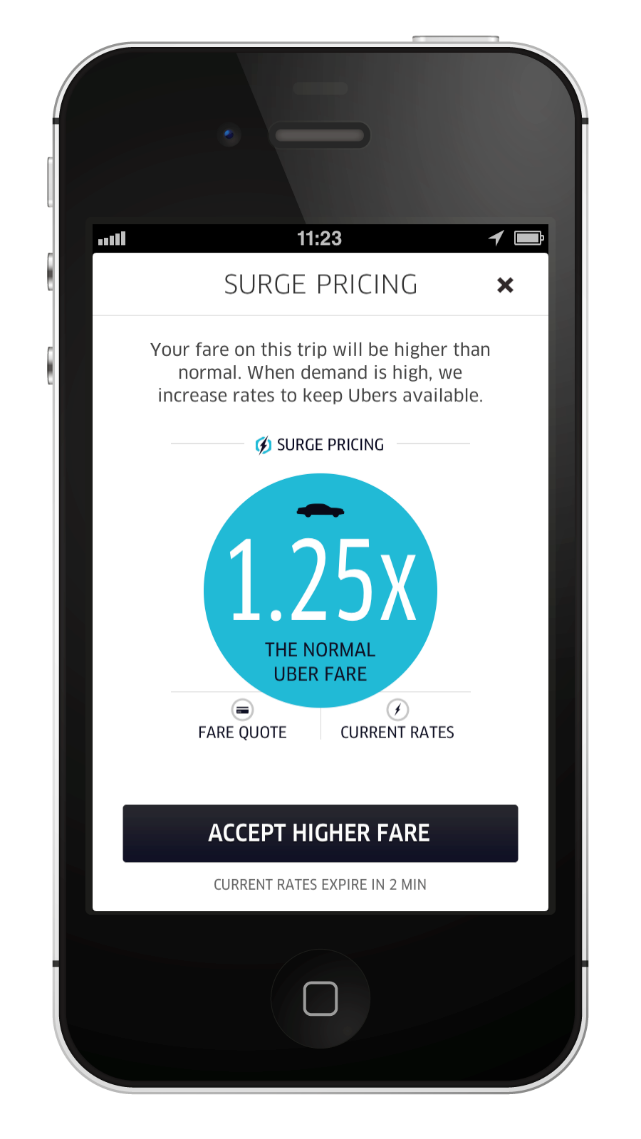
\includegraphics[width=7cm]{inc/surge_pricing.png}
            \caption[Surge Pricing]{Surge Pricing~\parencite{uber2013}}
            \label{fig:surge_pricing}
          \end{minipage}
        \end{figure}

        Uber's pricing algorithm automatically detects situations of high demand and low supply, increasing the price of the journey depending on the scale of the shortage~\parencite{dan2014}. The price hike encourages more drivers to work when needed. This method of Big Data-informed pricing is similar to that used by hotel chains and airlines to adjust rates to meet demand. However, rather than simply increasing prices at weekends or holidays, it uses predictive modelling to estimate demand in real-time~\parencite{marr2015}. Furthermore, unlike hotel rooms, the supply of Uber drivers is never always fixed, and according to~\cite{gurley2014} (A Deeper Look at Uber's Dynamic Pricing Model), most drivers would prefer not to be working at busy times.

      \subsection{UberPool}\label{subsec:uber_pool}

        \begin{figure}
          \centering
          \begin{minipage}{10cm}
            \centering
            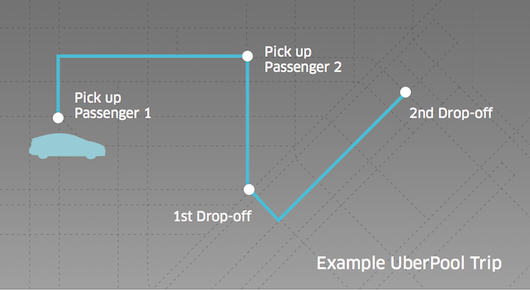
\includegraphics[width=10cm]{inc/uber_pool.png}
            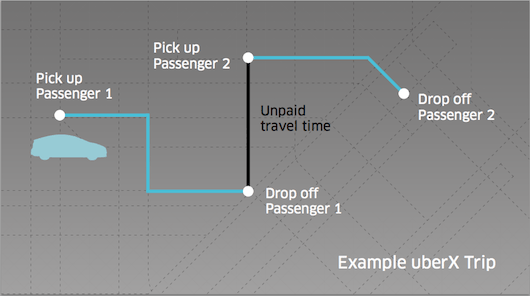
\includegraphics[width=10cm]{inc/uber_x.png}
            \caption[UberPool v.s.\ UberX]{UberPool v.s.\ UberX~\parencite{uber2014}}
            \label{fig:uber_pool_vs_uber_x}
          \end{minipage}
        \end{figure}

        Uber's car-pooling service UberPool allows users to find others near to them, which according to Uber's data, make similar journeys at similar times. Once a match has been found, users can decide to opt in or out of the carpool. \cite{iod2014} said that the service raised the prospect of a perpetual trip, describing it as ``the trip that never ends… the driver picks one passenger up, picks another passenger up, drops off the first passenger, but then picks up passenger number three and drops off passenger number two\ldots when this is really liquid that driver will always be carrying somebody''.

      \subsection{Rating Systems}\label{subsec:rating_systems}

        Uber's service relies on a detailed rating system -- users and drivers can rate each other in order to build up trust and help both parties to make decisions about who they want to share a ride with~\parencite{marr2015}. When a driver falls below a certain rating threshold their account is deactivated~\parencite{cook2015}.

      \subsection{Patent Applications}\label{subec:patent_applications}

        Uber has filed a number of patents, but according to \cite{decker2014}, many of them have been rejected by the U.S Patent and Trademark Office for ``obviousness''. Most of the company's patent applications appear to be for standard business models that have been around for a long time.

        \begin{figure}
          \centering
          \begin{minipage}{8cm}
            \centering
            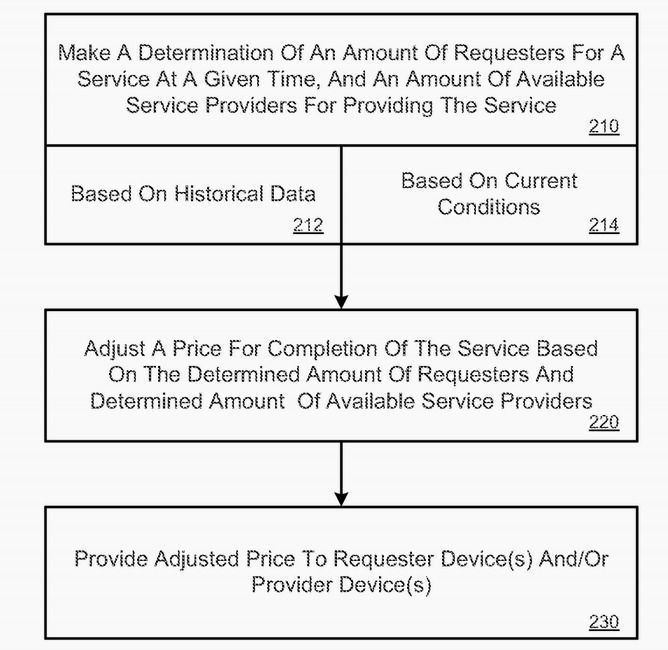
\includegraphics[width=8cm]{inc/patent_for_surge_pricing.png}
            \caption[Patent for Surge Pricing]{Patent for Surge Pricing~\parencite{}}
            \label{fig:patent_for_surge_pricing}
          \end{minipage}
        \end{figure}

        For example, it could be argued that Uber's surge pricing algorithm discussed in section~\ref{subsec:surge_pricing} (cf. Figure~\ref{fig:uber_pool_vs_uber_x}) simply involves using a computer to do a type of pricing that businesses have done for decades.

      \subsection{Allegations of Data Misuse}\label{subsec:allegations_of_data_misuse}

        Uber has been accused of having a casual disregard for user privacy on a number of occasions. For example, the launch party of Uber Chicago featured a screen that showed where certain ``known'' individuals were currently riding in Uber cabs. The usage of consumers’ personal information for ``entertainment purposes'' equates to the illegal sharing of location information, and Uber breaching its contract with its users~\parencite{sims2014}. Moreover, it raises a morality question of the ease at which a malicious Uber employee could start stalking particular users' if they had access to this `God View' tool, especially in connection to Michael's comments, which were espoused in section~\ref{sec:economic_conceptions} In the past, the company's executives have used the tool to index trips taken in Uber cars by journalists -- with two former employees describing the procedure of tracking customers as very easy~\parencite{canedo2014}.

        \begin{figure}
          \centering
          \begin{minipage}{10cm}
            \centering
            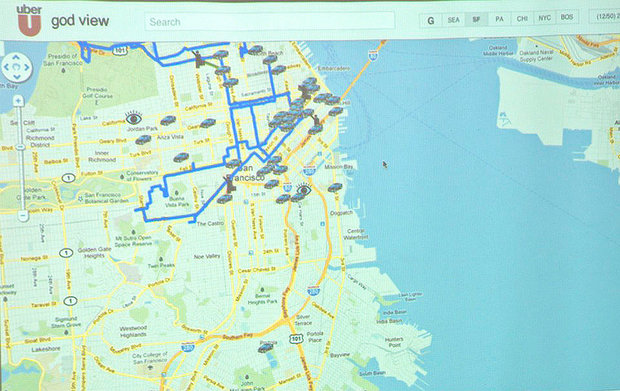
\includegraphics[width=10cm]{inc/god_view_tool.png}
            \caption[`God View' Tool]{`God View' Tool~\parencite{uber2011}}
            \label{fig:god_view_tool}
          \end{minipage}
        \end{figure}

        Correspondingly, the launch of the company's Uber Partner app contained a design flaw which gave all Uber driver's access to nearly $1\,000$ sensitive scanned documents (cf.\ Figure~\ref{fig:uber_data_breach}). In May 2014, a database containing the details of thousands of drivers was hacked and Uber did not notice until September. Even then, it did not notify any drivers that their details were at risk~\parencite{mccallion2015}.

        \begin{figure}
          \centering
          \begin{minipage}{10cm}
            \centering
            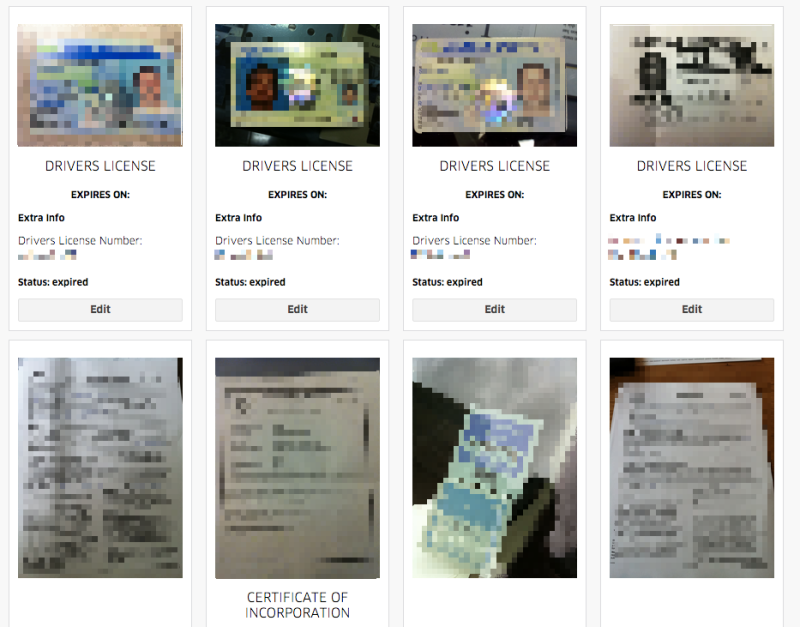
\includegraphics[width=10cm]{inc/uber_data_breach.png}
            \caption[Uber Data Breach]{Uber Data Breach~\parencite{biddle2015}}
            \label{fig:uber_data_breach}
          \end{minipage}
        \end{figure}

  \section{Key People}\label{sec:key_people}

    There were a few key individuals who, alongside Kalanick, have helped develop Uber as a company:

    \subsection{Ryan Graves, Head of Global Operations}\label{subsec:ryan_graves}

      Ryan Graves has been at Uber since launch, and has overseen the company's growth from 1 to 200+ employees. He has a background in organisation scaling, business development, product management and corporate restructuring~\parencite{crunchbase2015}.

    \subsection{Thuan Pham, Chief Technology Officer}\label{subsec:thuan_pham}

      Thuan Pham, was hired in April 2013, and is responsible for making technology decisions at Uber. He has been described as good at providing feedback, and capable of pushing himself and others to execute and grow beyond current limitations~\parencite{keyani2015}.

    \subsection{Salle Yoo, General Counsel}\label{subsec:salle_yoo}

      Salle Yoo, was hired in July 2012, and is responsible for managing Uber's legal and regulatory issues, especially when entering new markets, a process which has proven to be challenging for the company as it faces scrutiny in cities with strict transport laws. According to Yoo: ``when you go into an industry that hasn't seen innovation in 100 years and you bring a product that the regulations have not addressed\ldots there is going to be a period of time where you have to educate on what you are as a company and the value that you bring''~\parencite{johnson2015}.

  \section{Networks}\label{sec:networks}

    In terms of networking, Kalanick initially relied on Camp's business nous which helped launch Uber (as discussed in section~\ref{sec:economic_conceptions} and~\ref{sec:sociological_sonceptions}). Over time, the company has announced partnerships with:

    \subsection{Morgan Stanley}\label{subsec:morgan_stanley}

      Uber has been included in the aforementioned investment bank's corporate travel policy as the recommended transportation option for all employees~\parencite{uber2014b}. As a potentially lucrative IPO looms for the company, currently valued at \$50 billion, this could be viewed as an attempt by Morgan Stanley to demonstrate a more thorough familiarity with the service in order to increase the likelihood of being selected as the lead underwriter~\parencite{popper2015}.

    \subsection{Carnegie Mellon University}\label{subsec:carnegie_mellon_university}

      Initially, Carnegie Mellon and Uber trumpeted a collaborative partnership, which involved the institution working closely with the ride-hailing service to develop driverless car technologies. However, the tie-up quickly became more combative, as Uber poached 40 of the institution's researchers and scientists to staff the company's new R\&D centre in Pittsburgh. Uber envisions that autonomous cars will one day replace its contract drivers, and Carnegie Mellon's National Robotics Engineering Training Centre was picked by the company as the one place with enough talent to build the required team instantly~\parencite{ramsey2015}.

    \subsection{Hilton Worldwide}\label{subsec:hilton_worldwide}

      Hilton teamed up with Uber to increase the functionality of its app, Honors. The app now makes use of anonymised data from Uber to recommend the most popular venues to guests and act as travel guide, as well as allowing users to request rides~\parencite{kokalitcheva2015}.

    \subsection{Intact Worldwide}\label{subsec:intact_worldwide}

      Intact teamed up with Uber to create an insurance policy geared towards ride-sharing services to better legally protect drivers in case of a motor accident~\parencite{owram2015}.

      \begin{figure}
        \centering
        \begin{minipage}{14cm}
          \centering
          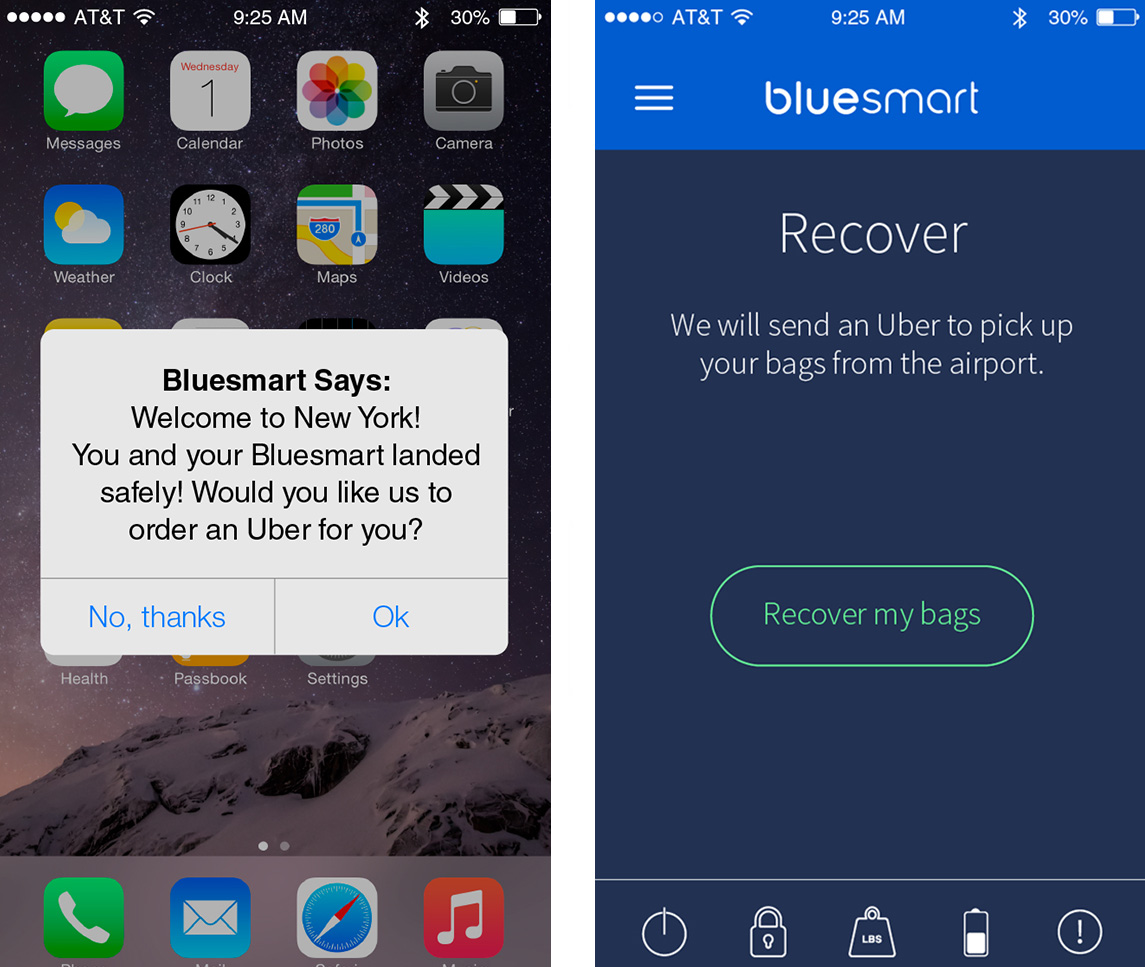
\includegraphics[width=14cm]{inc/bluesmart_uber_integration.png}
          \caption[Bluesmart Uber Integration]{Bluesmart Uber Integration~\parencite{bluesmart2015}}
          \label{fig:bluesmart_uber_integration}
        \end{minipage}
      \end{figure}

    \subsection{Bluesmart}\label{subsec:bluesmart}

      Bluesmart teamed up Uber to make it easier for smart luggage owners to reunite with their suitcases if they go astray, by sending an Uber driver to the airport to pick up the missing luggage and delivering it to the user's house as quickly as possible. Furthermore, Bluesmart's upcoming app will include a ``Request an Uber'' feature, which will use the suitcase's GPS tracker to detect when its owner has landed in an airport, and if this is the case, will automatically start searching for available cars and ask the user if they want an Uber ordered for them~\parencite{heim2015}.

  \section{Physical Resources}\label{sec:physical_resources}

    As Uber isn't a taxi company, but a service that connects passengers to drivers, then it does not need to own any of its own vehicles. Consequently, Uber can be thought of as a layer that sits on top of a large supply system and acts as an intermediary service~\parencite{goodwin2015}. According to \parencite{panzarino2013} Leaked Uber Numbers, Which We've Confirmed, Point To Over \$1B Gross, \$213M Revenue. Uber processes around 1M requests every week, and completes 800k each week. In order to enable high availability and deliverability, the company has invested in data centres to improve their computing, storage and networking capacities. Furthermore, in order to accommodate a ballooning headcount as the company grows, Uber is planning to move to a new downtown San Francisco HQ.

  \section{Funding}\label{sec:funding}

    \begin{figure}
      \centering
      \begin{minipage}{12cm}
        \centering
        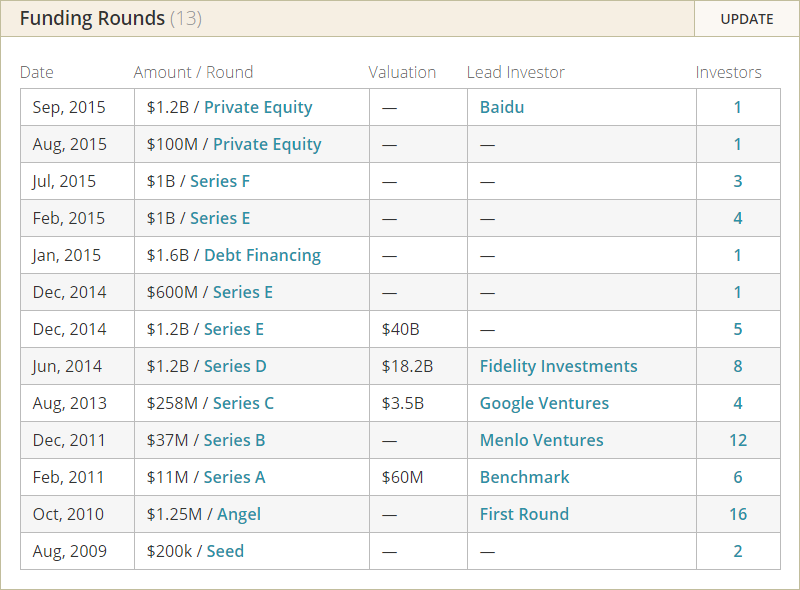
\includegraphics[width=12cm]{inc/uber_funding_rounds.png}
        \caption[Uber Funding Rounds]{Uber Funding Rounds~\parencite{}}
        \label{fig:uber_funding_rounds}
      \end{minipage}
    \end{figure}

    In August 2009, Uber received \$200k in funding from founders Kalanick and Camp which was used to develop the mobile app beta and test out their idea~\parencite{joshi2015}. Between October 2010 and September 2015 (cf.\ Figure~\ref{fig:uber_funding_rounds}), the company has raised \$10B in funding, setting a new record for a U.S.\ tech company. The fundraising has gone towards the company's expansion to more than 300 cities across the world, the cost of increasing legal fees, the development of new enterprise services and investment in technological innovations such as driverless cars~\parencite{bradshaw2015}. 
